\chapter{}\label{ex:aufg5}
%
\section{}\label{sec:aufg5a}
%
In der Abb.\ref{fig:drehzahldrehm} werden die Drehzahlen des BLDCs, bei den Ankerspannungen von $U_A = 20V$, $U_A = 15V$ und $U_A = 10V$, in Abhängigkeit des zu belastenden Drehmoments gezeigt.

\begin{figure}[htb]
	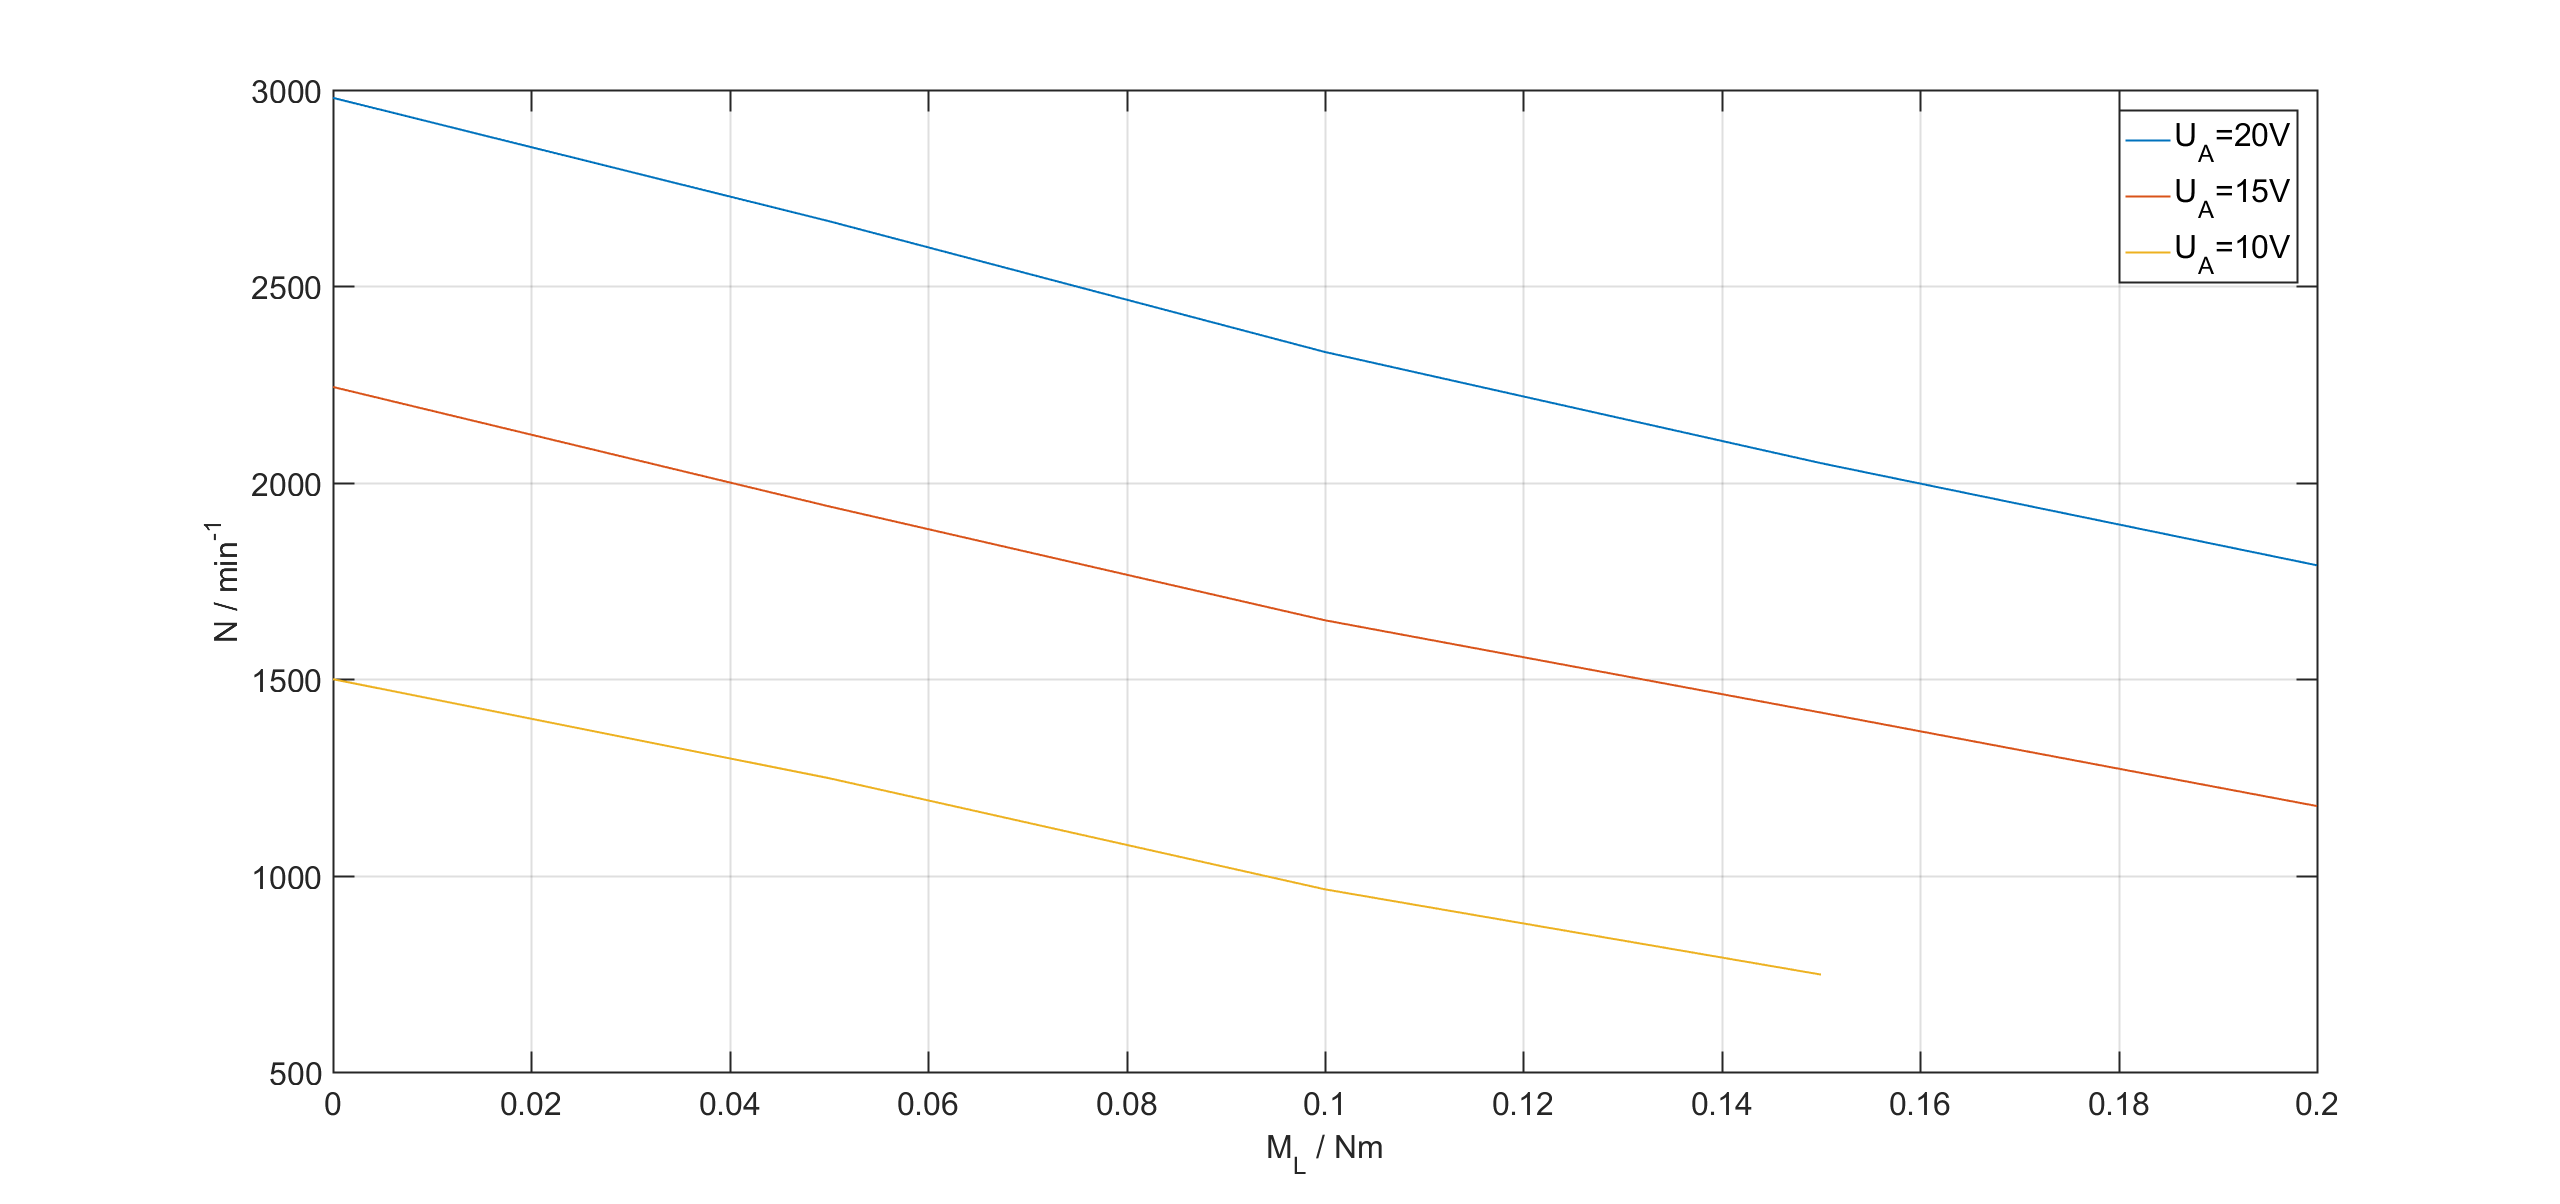
\includegraphics[width = \textwidth]{./Bilder/Drehzahldrehmomentkennlinie}
	\caption{Drehzahl-Drehmomentkennline}
	\label{fig:drehzahldrehm}
\end{figure}
%
\section{}\label{sec:aufg5b}
%
In Abb. \ref{fig:drehzahldrehm} erkennt man, dass bei einer Ankerspannung von $10V$ ein Drehmoment von $0.2 Nm$ nicht mehr erreicht werden kann. Dies rührt daher, dass der BLDC den DC-Motor antreibt und dieser somit generatorisch wirkt und eine Spannung erzeugt, welche wieder den Strom treibt. Durch den Laststrom-Regler wird nur der WIderstand der Gleichstrommaschine verändert. Bei $10V$ hat der BLDC eine bestimmte Drehzal, somit kann nur eine bestimmte Spannung am Generator erzeugt werden. Wenn der Widerstant minimal ist, dann fließt eben der maximal möglich Strom. Wenn die Drehzal absinkt ab auf $700 \frac{N}{min^{-1}}$, kann trotz minimalem Widerstand nur ein Strom von ca. $3A$ fließen.